% Created 2020-11-04 Wed 16:21
% Intended LaTeX compiler: pdflatex
\documentclass[11pt]{article}
\usepackage[utf8]{inputenc}
\usepackage[T1]{fontenc}
\usepackage{graphicx}
\usepackage{grffile}
\usepackage{longtable}
\usepackage{wrapfig}
\usepackage{rotating}
\usepackage[normalem]{ulem}
\usepackage{amsmath}
\usepackage{textcomp}
\usepackage{amssymb}
\usepackage{capt-of}
\usepackage{hyperref}
\author{Abram Hindle}
\date{\today}
\title{Survival Analysis}
\hypersetup{
 pdfauthor={Abram Hindle},
 pdftitle={Survival Analysis},
 pdfkeywords={},
 pdfsubject={},
 pdfcreator={Emacs 25.2.2 (Org mode 9.2.1)}, 
 pdflang={English}}
\begin{document}

\maketitle
\tableofcontents


\section{Survival Analysis}
\label{sec:orga24140f}
\subsection{Copyright Statement}
\label{sec:orgdc5389a}

If you are in CMPUT201 at UAlberta this code is released in the public
domain to you.

Otherwise it is (c) 2020 Abram Hindle

\subsubsection{License}
\label{sec:org931709a}

Survival Analysis
Copyright (C) 2020 Abram Hindle

This program is free software: you can redistribute it and/or modify
it under the terms of the GNU Affero General Public License as
published by the Free Software Foundation, either version 3 of the
License, or (at your option) any later version.

This program is distributed in the hope that it will be useful,
but WITHOUT ANY WARRANTY; without even the implied warranty of
MERCHANTABILITY or FITNESS FOR A PARTICULAR PURPOSE.  See the
GNU Affero General Public License for more details.

You should have received a copy of the GNU Affero General Public License
along with this program.  If not, see \url{https://www.gnu.org/licenses/}.

\subsubsection{Alternative version}
\label{sec:org845eaca}

Checkout the .txt, the .pdf, and the .html version

\subsubsection{Init ORG-MODE}
\label{sec:org7c47971}

\begin{verbatim}
;; I need this for org-mode to work well
;; If we have a new org-mode use ob-shell
;; otherwise use ob-sh --- but not both!
(if (require 'ob-shell nil 'noerror)
  (progn
    (org-babel-do-load-languages 'org-babel-load-languages '((shell . t))))
  (progn
    (require 'ob-sh)
    (org-babel-do-load-languages 'org-babel-load-languages '((sh . t)))))
(org-babel-do-load-languages
 'org-babel-load-languages
 '((R . t)))
(org-babel-do-load-languages 'org-babel-load-languages '((C . t)))
(org-babel-do-load-languages 'org-babel-load-languages '((python . t)))
(setq org-src-fontify-natively t)
(setq org-confirm-babel-evaluate nil) ;; danger!
(custom-set-faces
 '(org-block ((t (:inherit shadow :foreground "black"))))
 '(org-code ((t (:inherit shadow :foreground "black")))))
(setq org-startup-with-inline-images t)
(setq org-redisplay-inline-images t)
(add-hook 'org-babel-after-execute-hook 'org-display-inline-images)   
(add-hook 'org-mode-hook 'org-display-inline-images)   
\end{verbatim}


\subsubsection{Org export}
\label{sec:org6a191d3}
\begin{verbatim}
(org-html-export-to-html)
(org-latex-export-to-pdf)
(org-ascii-export-to-ascii)
\end{verbatim}


\subsubsection{Org Template}
\label{sec:org2c48a7b}

\begin{verbatim}
summary(runif(100))
\end{verbatim}

\begin{verbatim}
    Min.  1st Qu.   Median     Mean  3rd Qu.     Max. 
0.002381 0.171639 0.526952 0.516076 0.827670 0.986003
\end{verbatim}


\begin{verbatim}
library("ggplot2")
ggplot(iris, aes(x = Sepal.Width, y = Sepal.Length, color = Species)) +
geom_point()
\end{verbatim}

\begin{center}
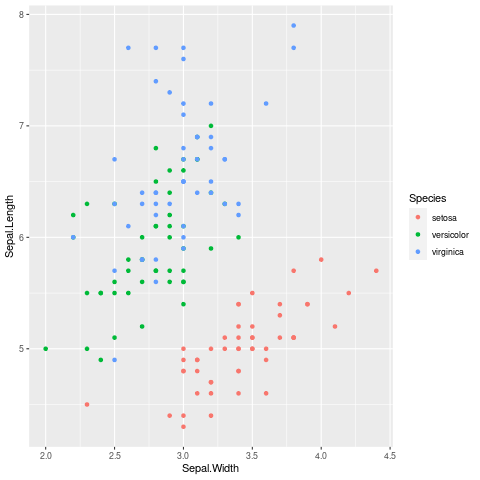
\includegraphics[width=.9\linewidth]{test.png}
\end{center}



\subsection{Survival Analysis}
\label{sec:org5aafdf0}
\url{https://github.com/therneau/survival}
\url{https://cran.r-project.org/web/packages/survival/index.html}
\url{https://cran.r-project.org/web/packages/survival/survival.pdf}
\subsubsection{Survival Data}
\label{sec:org8c77eb4}

Let's try it out from the R package

Let's look at what is expected from survival data:

\begin{verbatim}
library(survival)
aml
\end{verbatim}

\begin{verbatim}
   time status             x
1     9      1    Maintained
2    13      1    Maintained
3    13      0    Maintained
4    18      1    Maintained
5    23      1    Maintained
6    28      0    Maintained
7    31      1    Maintained
8    34      1    Maintained
9    45      0    Maintained
10   48      1    Maintained
11  161      0    Maintained
12    5      1 Nonmaintained
13    5      1 Nonmaintained
14    8      1 Nonmaintained
15    8      1 Nonmaintained
16   12      1 Nonmaintained
17   16      0 Nonmaintained
18   23      1 Nonmaintained
19   27      1 Nonmaintained
20   30      1 Nonmaintained
21   33      1 Nonmaintained
22   43      1 Nonmaintained
23   45      1 Nonmaintained
\end{verbatim}

Time is when an event occurs. Status is alive or dead. x is the factor.

This is Leukemia survival data.

\subsubsection{Surv object}
\label{sec:org0b7e58c}

survfit will fit a model to a survival curve. Surv makes such a curve out of 2 variables, time and status.

Status is either censoring or death. 0 for censor often, or 1 for death?

\begin{verbatim}
maint <- aml[aml$x=="Maintained",]
Surv(maint$time, maint$status)
maint[maint$status==0,]
\end{verbatim}

\begin{verbatim}
 [1]   9   13   13+  18   23   28+  31   34   45+  48  161+
   time status          x
3    13      0 Maintained
6    28      0 Maintained
9    45      0 Maintained
11  161      0 Maintained
\end{verbatim}

\subsubsection{Plotting Surv object}
\label{sec:orgca23d6c}

You can plot the curve and the confidence interval

\begin{verbatim}
maint <- aml[aml$x=="Maintained",]
plot(Surv(maint$time, maint$status))
\end{verbatim}

\begin{center}
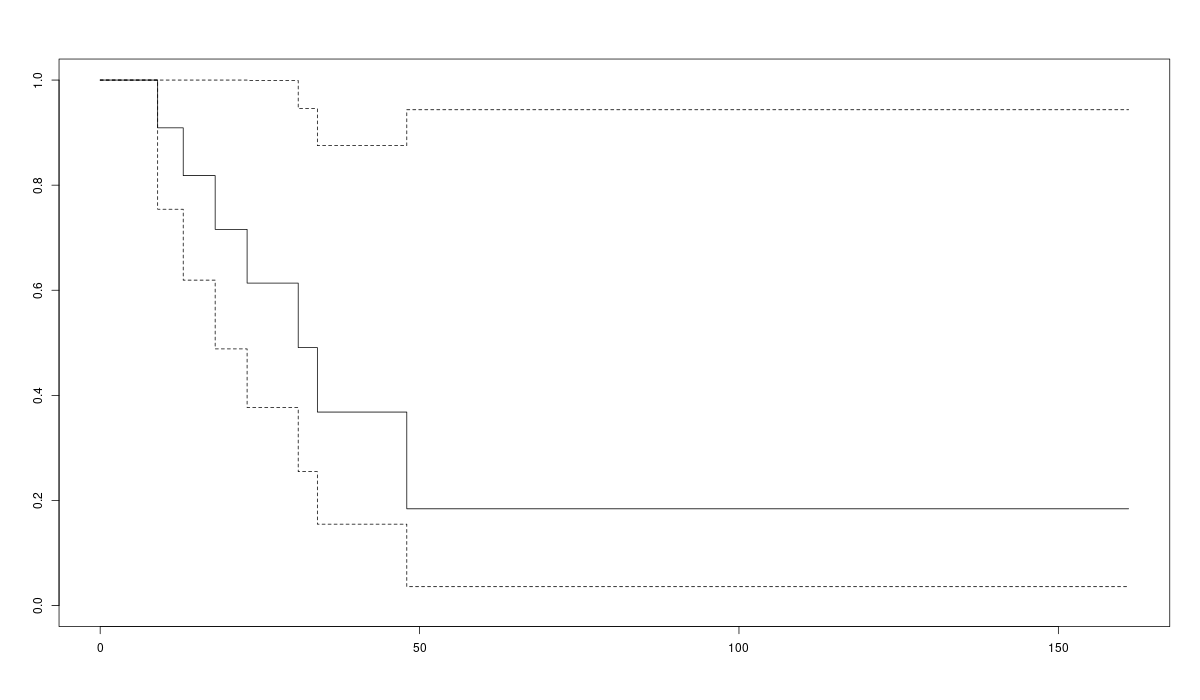
\includegraphics[width=.9\linewidth]{Surv.png}
\end{center}
So what does it look like with multiple factors?

\begin{verbatim}
leukemia.surv <- survfit(Surv(time, status) ~ x, data = aml)
plot(leukemia.surv, lty = 2:3)
legend(100, .9, c("Maintenance", "No Maintenance"), lty = 2:3)
\end{verbatim}

\begin{center}
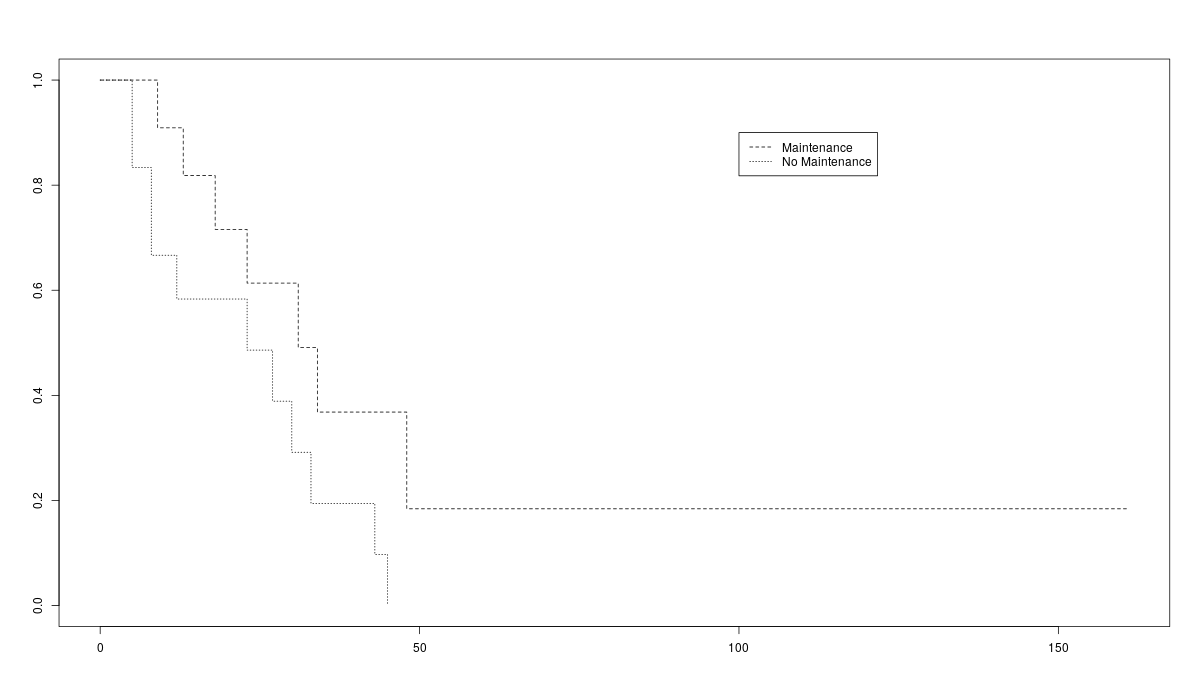
\includegraphics[width=.9\linewidth]{leukemia.png}
\end{center}

\begin{verbatim}
leukemia.surv <- survfit(Surv(time, status) ~ x, data = aml)
summary(leukemia.surv)
\end{verbatim}

\begin{verbatim}
Call: survfit(formula = Surv(time, status) ~ x, data = aml)

                x=Maintained 
 time n.risk n.event survival std.err lower 95% CI upper 95% CI
    9     11       1    0.909  0.0867       0.7541        1.000
   13     10       1    0.818  0.1163       0.6192        1.000
   18      8       1    0.716  0.1397       0.4884        1.000
   23      7       1    0.614  0.1526       0.3769        0.999
   31      5       1    0.491  0.1642       0.2549        0.946
   34      4       1    0.368  0.1627       0.1549        0.875
   48      2       1    0.184  0.1535       0.0359        0.944

                x=Nonmaintained 
 time n.risk n.event survival std.err lower 95% CI upper 95% CI
    5     12       2   0.8333  0.1076       0.6470        1.000
    8     10       2   0.6667  0.1361       0.4468        0.995
   12      8       1   0.5833  0.1423       0.3616        0.941
   23      6       1   0.4861  0.1481       0.2675        0.883
   27      5       1   0.3889  0.1470       0.1854        0.816
   30      4       1   0.2917  0.1387       0.1148        0.741
   33      3       1   0.1944  0.1219       0.0569        0.664
   43      2       1   0.0972  0.0919       0.0153        0.620
   45      1       1   0.0000     NaN           NA           NA
\end{verbatim}


\subsubsection{OK but software engineering?}
\label{sec:org982bf54}

Your times should be time since the start of the intervention or the
birth of a bug. If you want to track project lifetime, make it another
variable. Your record should be if something has quit or if something
has finished.

\begin{verbatim}
library(survival)
bugs <- c()
# time of bug fix
bugs$time   <- c(10,10,10,20,20,30,40,50,60,70,80,90,100)
# bugs$status <- c( 0, 0, 0, 0, 1, 0, 1, 0, 0, 1, 1, 0,  1)
bugs <- data.frame(bugs)
bugs
\end{verbatim}

\begin{verbatim}
   time
1    10
2    10
3    10
4    20
5    20
6    30
7    40
8    50
9    60
10   70
11   80
12   90
13  100
\end{verbatim}

\begin{verbatim}
plot(Surv(bugs$time))
\end{verbatim}

\begin{center}
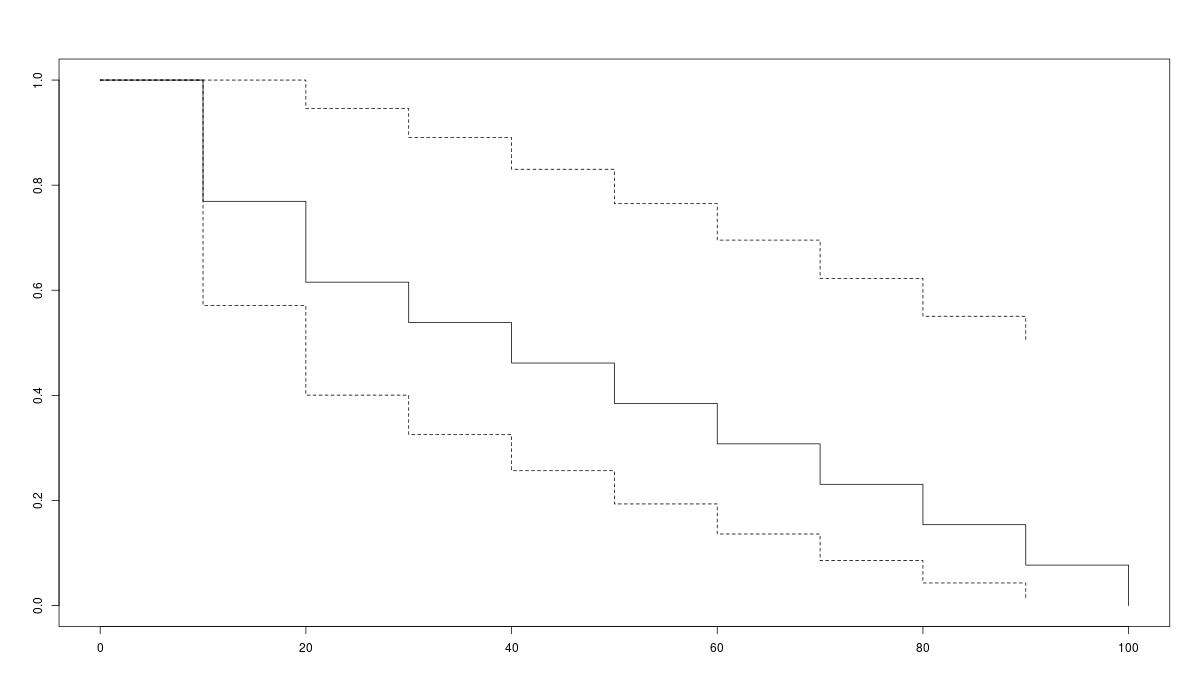
\includegraphics[width=.9\linewidth]{Bugs.png}
\end{center}

\subsubsection{What about for a lot more bugs?}
\label{sec:org4d521d7}

We're going to invent a dataset where minor revision bugs last longer.

They are fixed later. Which means they survive longer.

\begin{verbatim}
bugs <- c()
# bug survival
bugs$time   <- sort(runif(100)*100)
# longer surviving bugs at the end
bugs$time   <- c(bugs$time,sort(bugs$time + runif(100)*50))
# the first half are half minor revisions
# the second half are mostly minor revision bugs and they last a long time
bugs$minor  <- c(sample(c(0,1),100,replace=TRUE),sample(c(1),100,replace=TRUE))
# this is just noise to show what happens with uncorrelated results
bugs$noise  <- sample(c(0,1),200,replace=TRUE)
# minor are censored more
bugs$status <- c(sample(c(1,1,1,0),100,replace=TRUE),sample(c(1,0,0),100,replace=TRUE))
bugs <- data.frame(bugs)
# plot(bugs$time[bugs$status==1])
# plot(bugs$time[bugs$status==0])
plot(Surv(bugs$time,bugs$status))
\end{verbatim}

\begin{center}
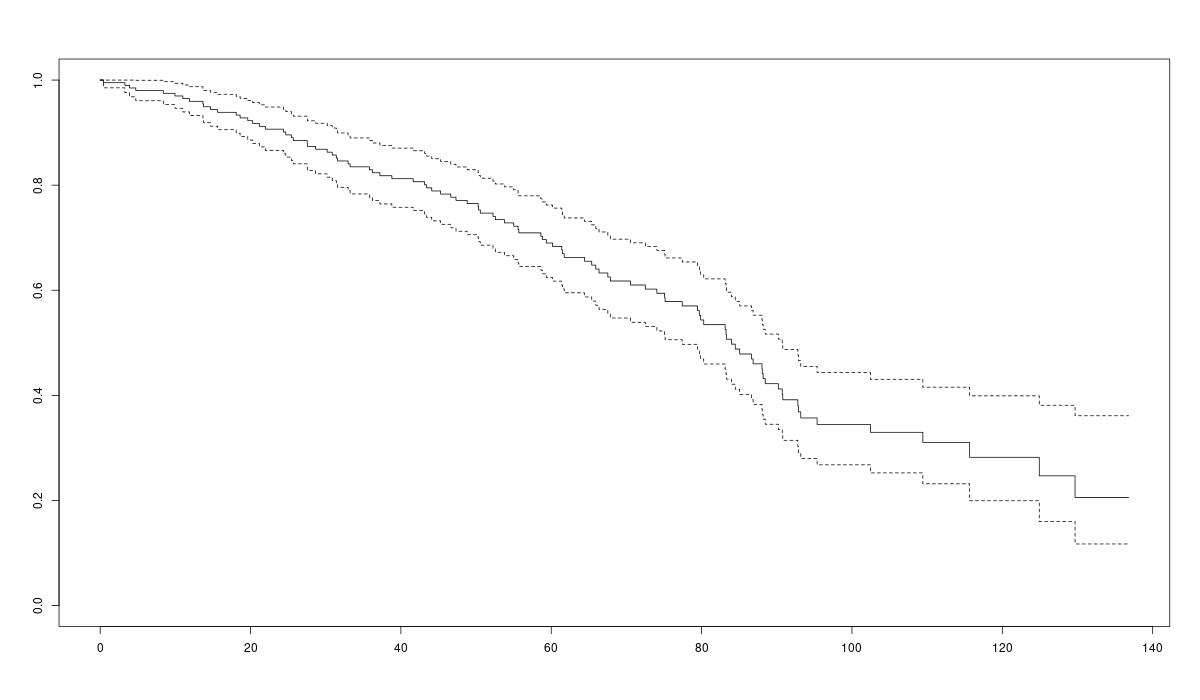
\includegraphics[width=.9\linewidth]{RandBugs.png}
\end{center}
\begin{verbatim}
plot(survfit(Surv(time,status) ~ factor(minor), data = bugs),lty=c(1:2))
legend(100, .9, c("Not minor", "Minor"), lty = 1:2)
\end{verbatim}

\begin{center}
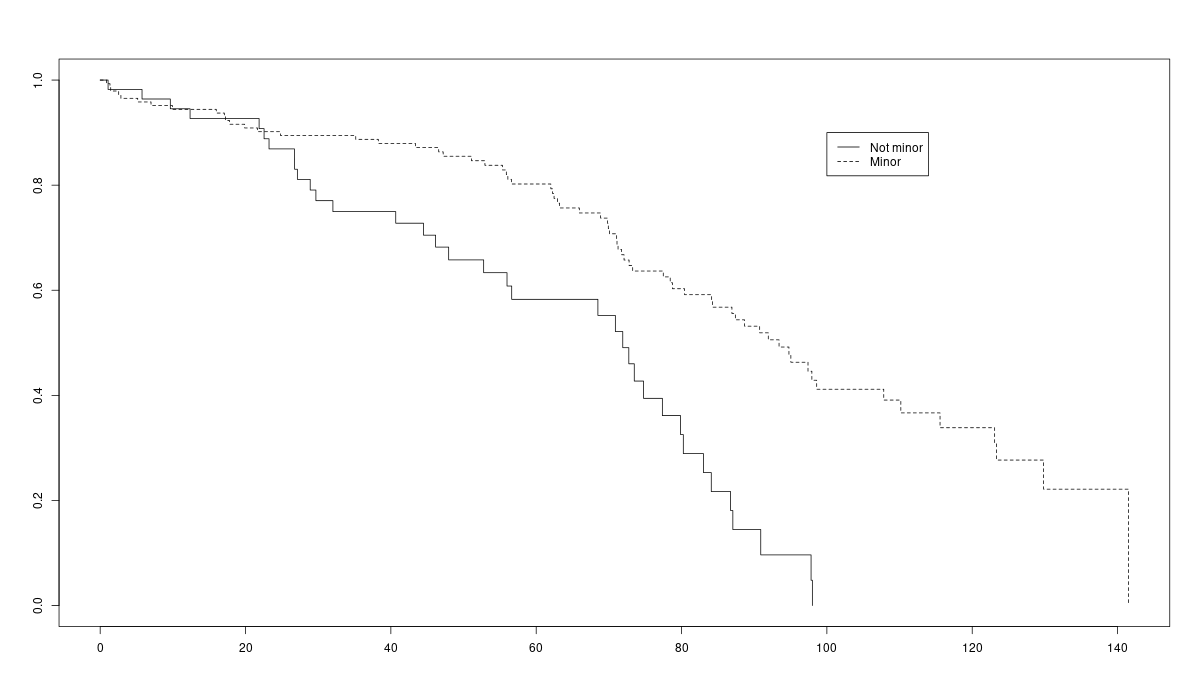
\includegraphics[width=.9\linewidth]{SurvFitRandBugs.png}
\end{center}
\begin{verbatim}
summary(survfit(Surv(time,status) ~ factor(minor), data = bugs))
\end{verbatim}

\begin{verbatim}
Call: survfit(formula = Surv(time, status) ~ factor(minor), data = bugs)

                factor(minor)=0 
  time n.risk n.event survival std.err lower 95% CI upper 95% CI
  1.81     44       1   0.9773  0.0225      0.93421        1.000
  4.50     43       1   0.9545  0.0314      0.89494        1.000
  5.26     42       1   0.9318  0.0380      0.86024        1.000
  7.28     41       1   0.9091  0.0433      0.82800        0.998
  9.10     39       1   0.8858  0.0481      0.79637        0.985
 11.74     38       1   0.8625  0.0522      0.76605        0.971
 12.52     37       1   0.8392  0.0557      0.73675        0.956
 15.41     35       1   0.8152  0.0591      0.70726        0.940
 15.88     34       1   0.7912  0.0620      0.67856        0.923
 18.71     33       1   0.7672  0.0646      0.65053        0.905
 19.51     32       1   0.7433  0.0669      0.62309        0.887
 22.66     29       1   0.7176  0.0693      0.59387        0.867
 25.41     28       1   0.6920  0.0714      0.56528        0.847
 28.29     27       1   0.6664  0.0732      0.53725        0.827
 37.46     25       1   0.6397  0.0750      0.50840        0.805
 39.38     24       1   0.6131  0.0765      0.48012        0.783
 40.89     22       1   0.5852  0.0779      0.45081        0.760
 42.76     21       1   0.5573  0.0790      0.42212        0.736
 43.60     20       1   0.5295  0.0798      0.39400        0.711
 45.51     18       1   0.5000  0.0806      0.36455        0.686
 52.09     17       1   0.4706  0.0811      0.33578        0.660
 54.66     16       1   0.4412  0.0812      0.30766        0.633
 55.48     15       1   0.4118  0.0809      0.28019        0.605
 57.32     13       1   0.3801  0.0806      0.25080        0.576
 58.38     12       1   0.3484  0.0799      0.22230        0.546
 75.69      9       1   0.3097  0.0799      0.18686        0.513
 76.95      8       1   0.2710  0.0787      0.15339        0.479
 77.40      7       1   0.2323  0.0764      0.12193        0.443
 83.70      6       1   0.1936  0.0728      0.09262        0.405
 93.28      4       1   0.1452  0.0688      0.05732        0.368
 95.40      3       1   0.0968  0.0606      0.02840        0.330
 95.79      2       1   0.0484  0.0457      0.00761        0.308
 96.67      1       1   0.0000     NaN           NA           NA

                factor(minor)=1 
   time n.risk n.event survival std.err lower 95% CI upper 95% CI
   1.80    154       1    0.994 0.00647        0.981        1.000
   3.07    153       1    0.987 0.00912        0.969        1.000
   3.13    152       1    0.981 0.01114        0.959        1.000
   4.35    151       1    0.974 0.01282        0.949        0.999
   4.86    150       1    0.968 0.01428        0.940        0.996
  10.11    148       1    0.961 0.01561        0.931        0.992
  10.34    147       1    0.954 0.01682        0.922        0.988
  13.67    143       1    0.948 0.01798        0.913        0.984
  21.87    135       1    0.941 0.01916        0.904        0.979
  22.48    134       1    0.934 0.02027        0.895        0.974
  24.12    132       1    0.927 0.02131        0.886        0.969
  24.45    131       1    0.920 0.02229        0.877        0.964
  26.56    129       1    0.912 0.02323        0.868        0.959
  26.70    128       1    0.905 0.02412        0.859        0.954
  28.85    125       1    0.898 0.02499        0.850        0.948
  30.93    124       1    0.891 0.02582        0.842        0.943
  34.37    123       1    0.884 0.02660        0.833        0.937
  35.80    121       1    0.876 0.02737        0.824        0.932
  36.13    119       1    0.869 0.02811        0.816        0.926
  36.15    118       1    0.862 0.02882        0.807        0.920
  36.66    117       1    0.854 0.02950        0.798        0.914
  37.51    116       1    0.847 0.03015        0.790        0.908
  38.23    115       1    0.839 0.03077        0.781        0.902
  39.57    114       1    0.832 0.03137        0.773        0.896
  41.51    111       1    0.825 0.03197        0.764        0.890
  43.08    109       1    0.817 0.03256        0.756        0.883
  43.23    108       1    0.809 0.03313        0.747        0.877
  45.28    107       1    0.802 0.03367        0.739        0.871
  47.88    105       1    0.794 0.03421        0.730        0.864
  48.09    104       1    0.787 0.03472        0.721        0.858
  48.11    103       1    0.779 0.03521        0.713        0.851
  49.19    101       1    0.771 0.03570        0.704        0.845
  50.69     97       1    0.763 0.03621        0.696        0.838
  51.06     95       1    0.755 0.03671        0.687        0.831
  51.30     94       1    0.747 0.03718        0.678        0.824
  51.40     93       1    0.739 0.03764        0.669        0.817
  51.53     92       1    0.731 0.03808        0.660        0.810
  51.77     91       1    0.723 0.03850        0.652        0.803
  52.01     90       1    0.715 0.03890        0.643        0.796
  53.30     89       1    0.707 0.03929        0.634        0.788
  58.49     80       1    0.698 0.03978        0.624        0.781
  58.81     79       1    0.689 0.04024        0.615        0.773
  59.64     77       1    0.680 0.04071        0.605        0.765
  60.76     75       1    0.671 0.04116        0.595        0.757
  61.55     74       1    0.662 0.04159        0.586        0.749
  70.07     66       1    0.652 0.04216        0.575        0.740
  71.11     63       1    0.642 0.04274        0.563        0.731
  75.05     60       1    0.631 0.04335        0.552        0.722
  75.78     59       1    0.621 0.04391        0.540        0.713
  75.93     58       1    0.610 0.04444        0.529        0.703
  77.52     56       1    0.599 0.04496        0.517        0.694
  78.09     55       1    0.588 0.04544        0.505        0.684
  80.36     53       1    0.577 0.04592        0.494        0.674
  80.47     52       1    0.566 0.04636        0.482        0.664
  81.87     51       1    0.555 0.04676        0.470        0.654
  84.11     49       1    0.543 0.04715        0.458        0.644
  84.82     48       1    0.532 0.04751        0.447        0.634
  85.09     47       1    0.521 0.04783        0.435        0.624
  89.86     41       1    0.508 0.04832        0.422        0.612
  92.47     38       1    0.495 0.04886        0.408        0.600
  96.46     32       1    0.479 0.04972        0.391        0.587
  96.56     30       1    0.463 0.05057        0.374        0.574
  97.75     28       1    0.447 0.05140        0.357        0.560
  97.76     27       1    0.430 0.05209        0.339        0.545
  99.06     24       1    0.412 0.05291        0.321        0.530
 100.28     23       1    0.394 0.05356        0.302        0.515
 102.84     21       1    0.376 0.05420        0.283        0.498
 104.95     19       1    0.356 0.05484        0.263        0.481
 105.31     18       1    0.336 0.05524        0.243        0.464
 108.29     15       1    0.314 0.05591        0.221        0.445
 112.26     10       1    0.282 0.05846        0.188        0.424
 126.96      4       1    0.212 0.07522        0.106        0.425
\end{verbatim}

Survfit basically calculates confidence intervals of survival at each point


\subsubsection{Cox Proportional-Hazards Model}
\label{sec:org32aba7a}

The PMM for minor should be lower than not minor. Because it is less risk. It lets bugs survive longer.

The PMM for noise should be near 1.

\begin{verbatim}
fit <- coxph(Surv(time,status) ~ factor(minor) + factor(noise), data = bugs)
summary(fit,rr.ci=TRUE)
yates(fit, ~ minor, predict="risk") # hazard ratio
yates(fit, ~ noise, predict="risk") # hazard ratio
\end{verbatim}

\begin{verbatim}
Call:
coxph(formula = Surv(time, status) ~ factor(minor) + factor(noise), 
    data = bugs)

  n= 200, number of events= 105 

                  coef exp(coef) se(coef)      z Pr(>|z|)    
factor(minor)1 -1.0992    0.3331   0.2189 -5.022 5.13e-07 ***
factor(noise)1  0.1994    1.2206   0.1973  1.010    0.312    
---
Signif. codes:  0 ‘***’ 0.001 ‘**’ 0.01 ‘*’ 0.05 ‘.’ 0.1 ‘ ’ 1

               exp(coef) exp(-coef) lower .95 upper .95
factor(minor)1    0.3331     3.0018    0.2169    0.5116
factor(noise)1    1.2206     0.8193    0.8291    1.7970

Concordance= 0.613  (se = 0.03 )
Likelihood ratio test= 23.37  on 2 df,   p=8e-06
Wald test            = 26.7  on 2 df,   p=2e-06
Score (logrank) test = 29.34  on 2 df,   p=4e-07
 factor(minor)     pmm      std               test chisq df        Pr
             0 2.35565 0.426003      factor(minor) 11.41  1 0.0007322
             1 0.78475 0.041541
 factor(noise)    pmm     std               test  chisq df     Pr
             0 1.0375 0.10730      factor(noise) 0.9356  1 0.3334
             1 1.2664 0.15896
\end{verbatim}

\begin{verbatim}
fit <- coxph(Surv(time,status) ~ factor(minor) + factor(noise), data = bugs)
par(mfrow=c(3,1))
plot(cox.zph(fit)[1]) # plot minor
plot(cox.zph(fit)[2]) # plot noise
plot(survfit(Surv(time,status) ~ factor(minor), data = bugs),lty=c(1:2))
legend(100, .9, c("Not minor", "Minor"), lty = 1:2)
\end{verbatim}

\begin{center}
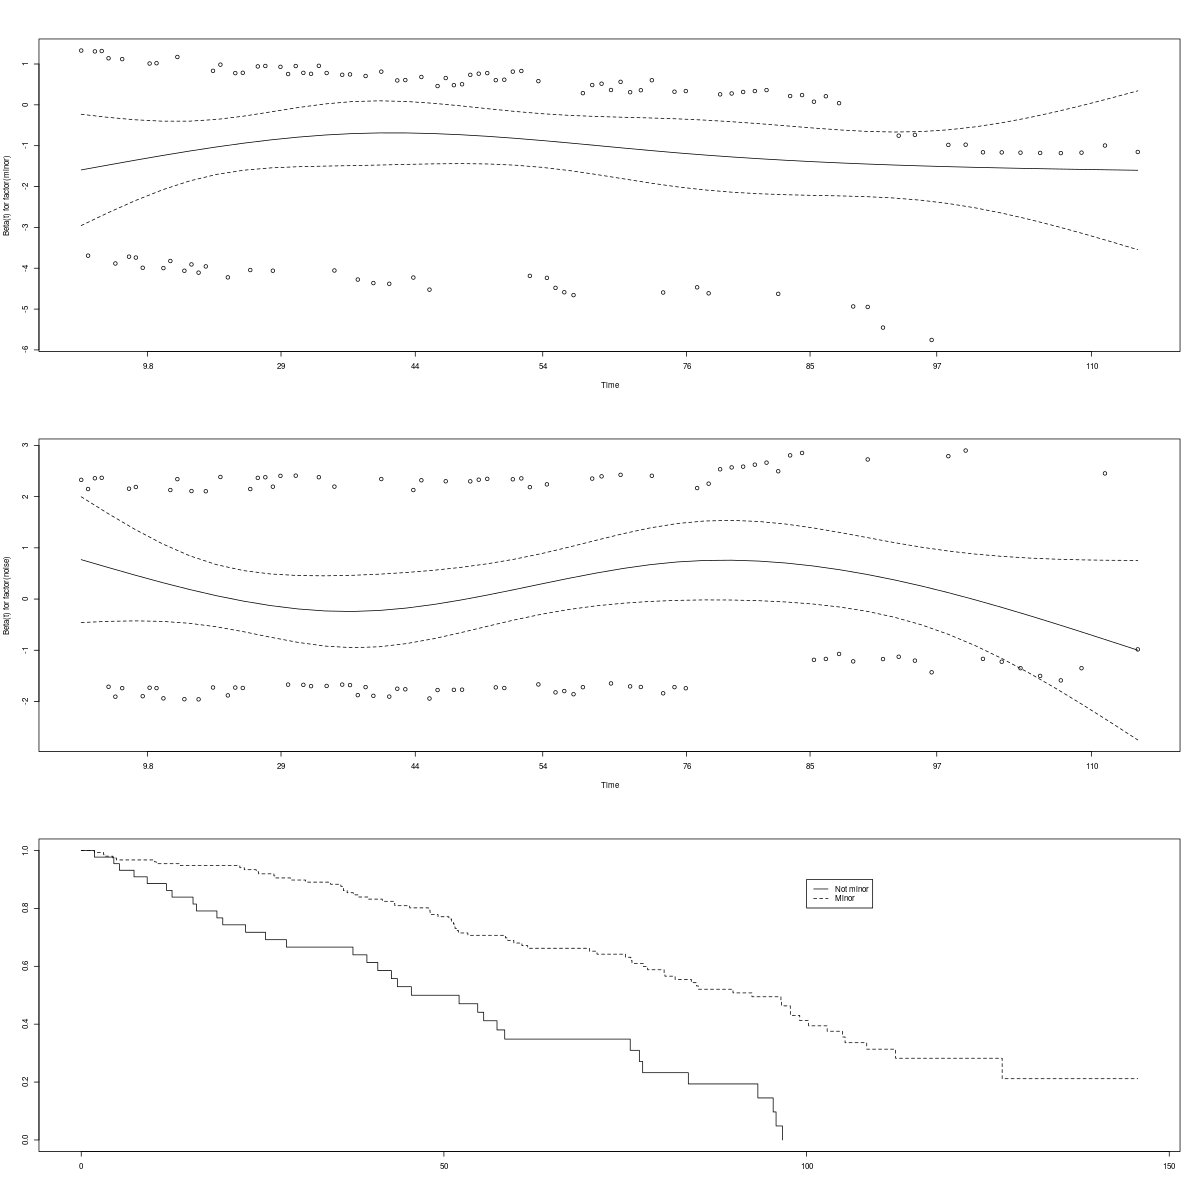
\includegraphics[width=.9\linewidth]{RandBugsCox.png}
\end{center}
\subsubsection{Pretty Plots with Survminer}
\label{sec:org2d670db}

A pain to install (use docker?) \url{https://rpkgs.datanovia.com/survminer/}

You could install devtools and run:

\begin{verbatim}
devtools::install_url("https://github.com/wilkelab/cowplot/archive/0.6.3.zip")
devtools::install_url("https://github.com/cran/mvtnorm/archive/1.0-8.zip")
devtools::install_url("https://github.com/kassambara/survminer/archive/v0.4.3.zip")
#install.packages("survminer")
\end{verbatim}

\begin{verbatim}
library(survminer)
\end{verbatim}

\begin{verbatim}
library(survival)
library(survminer)
fit <- survfit(Surv(time,status) ~ factor(minor), data = bugs)
ggsurvplot(fit, data = bugs)
\end{verbatim}

\begin{center}
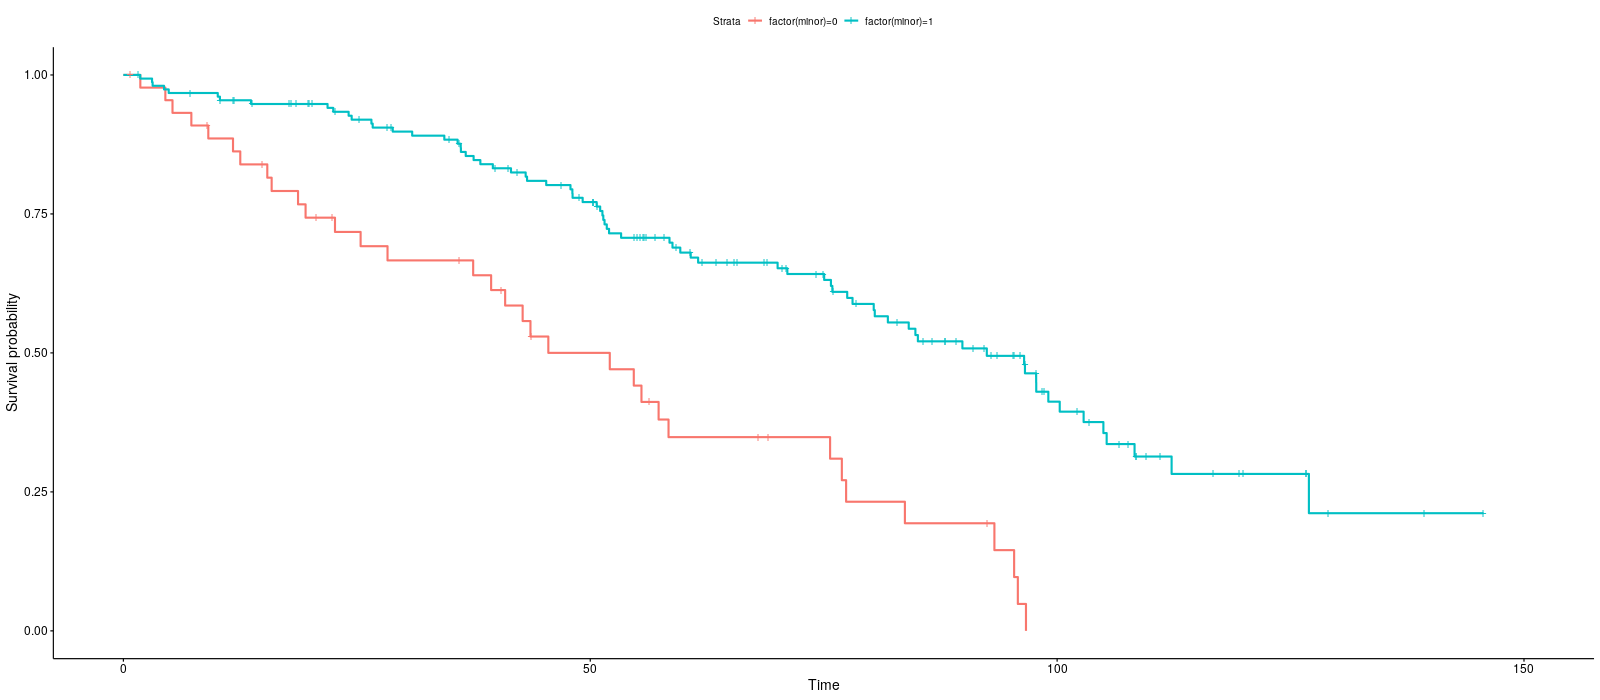
\includegraphics[width=.9\linewidth]{SurvMinerRandBugsCox.png}
\end{center}
\subsubsection{Better}
\label{sec:orge24a2be}


\begin{verbatim}
library(survival)
library(survminer)
fit <- survfit(Surv(time,status) ~ factor(minor), data = bugs)
ggsurvplot(
  fit, 
  data = bugs, 
  size = 1,                 # change line size
  palette = 
    c("#E7B800", "#2E9FDF"),# custom color palettes
  conf.int = TRUE,          # Add confidence interval
  pval = TRUE,              # Add p-value
  risk.table = TRUE,        # Add risk table
  risk.table.col = "strata",# Risk table color by groups
  legend.labs = 
    c("Not Minor", "Minor"),    # Change legend labels
  risk.table.height = 0.25, # Useful to change when you have multiple groups
  ggtheme = theme_bw()      # Change ggplot2 theme
)
\end{verbatim}

\begin{center}
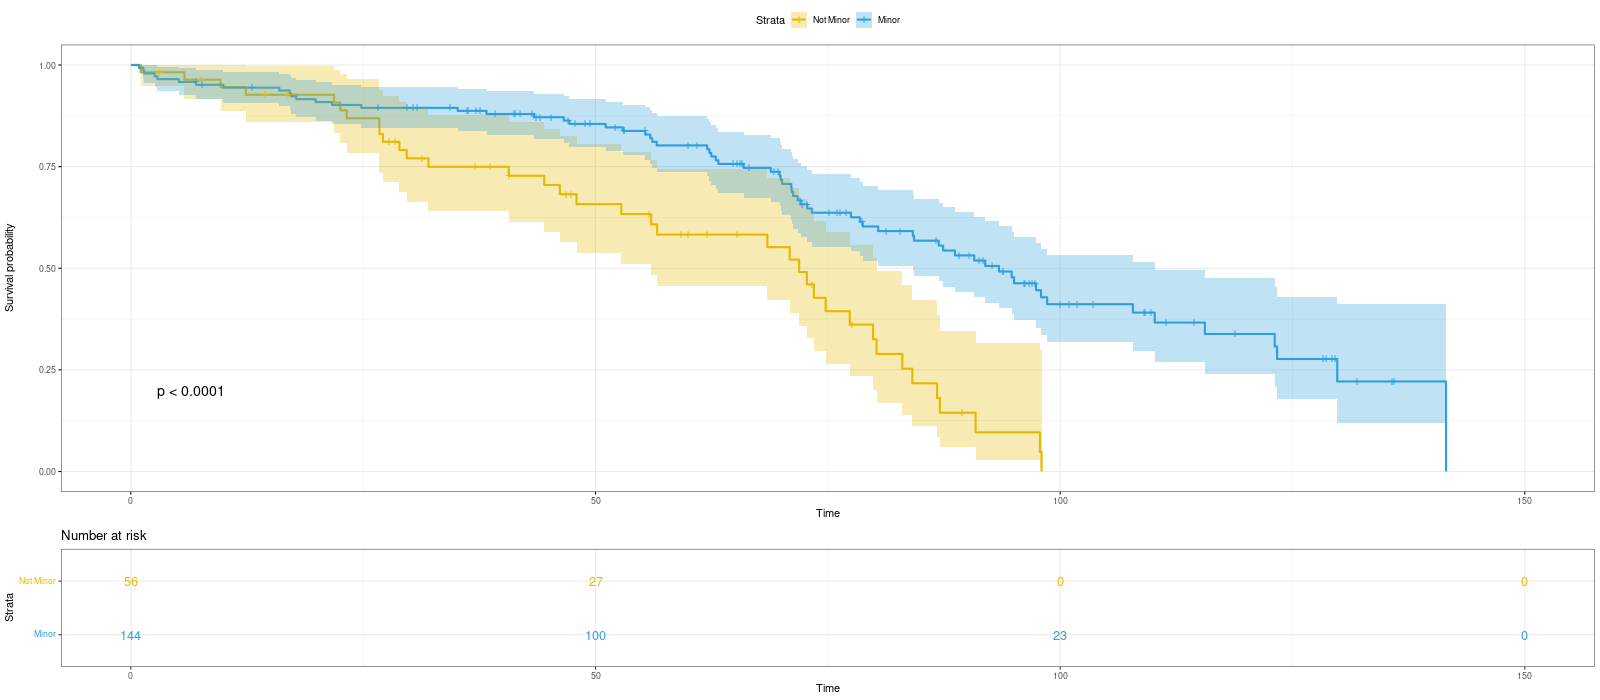
\includegraphics[width=.9\linewidth]{PrettySurvMinerRandBugsCox.png}
\end{center}
\end{document}
